 \begin{figure}
\center

Ground Truth: $p = 8$

Example 1

\begin{minipage}[c]{0.8\linewidth}
\sideimage{Fitted}{figures/CounterfactualModel_VIZ.py_12345_FOURIER_181_FOURIER_281_8_0_10.0_180.pdf}

\sideimage{Fitted}{figures/RunSynthetic_FreePrior_CosineLoss_OnSim_VIZ.py_SimulateSynthetic_Parameterized_OtherNoiseLevels_Grid_VarySize.py_180_8_2345_N10000_FOURIER_181_FOURIER_281.txt_8_0_10.0_180.pdf}
\end{minipage}
\begin{minipage}[c]{0.19\linewidth}
\centering

\ \ \ \ \ \ Negative

\ \ \ \ \ \ Log-Likelihood

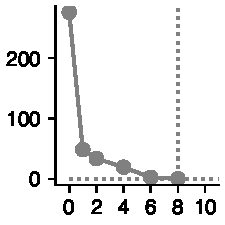
\includegraphics[width=0.98\textwidth]{figures/evaluateCrossValidationResults_Synthetic_Gardelle.py_SimulateSynthetic_Parameterized_OtherNoiseLevels_Grid_VarySize.py_180_8_2345_N10000_FOURIER_181_FOURIER_281.txt_RelativeLF.pdf}
\end{minipage}

\ 

Example 2

\begin{minipage}[c]{0.8\linewidth}
\sideimage{Fitted}{figures/CounterfactualModel_VIZ.py_12345_FOURIER_182_FOURIER_282_8_0_10.0_180.pdf}

\sideimage{Fitted}{figures/RunSynthetic_FreePrior_CosineLoss_OnSim_VIZ.py_SimulateSynthetic_Parameterized_OtherNoiseLevels_Grid_VarySize.py_180_8_2345_N10000_FOURIER_182_FOURIER_282.txt_8_0_10.0_180.pdf}
\end{minipage}
\begin{minipage}[c]{0.19\linewidth}
\centering

\ \ \ \ \ \ Negative

\ \ \ \ \ \ Log-Likelihood

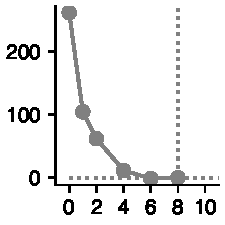
\includegraphics[width=0.98\textwidth]{figures/evaluateCrossValidationResults_Synthetic_Gardelle.py_SimulateSynthetic_Parameterized_OtherNoiseLevels_Grid_VarySize.py_180_8_2345_N10000_FOURIER_182_FOURIER_282.txt_RelativeLF.pdf}
\end{minipage}

\ 

Example 3

\begin{minipage}[c]{0.8\linewidth}
\sideimage{Fitted}{figures/CounterfactualModel_VIZ.py_12345_FOURIER_183_FOURIER_283_8_0_10.0_180.pdf}

\sideimage{Fitted}{figures/RunSynthetic_FreePrior_CosineLoss_OnSim_VIZ.py_SimulateSynthetic_Parameterized_OtherNoiseLevels_Grid_VarySize.py_180_8_2345_N10000_FOURIER_183_FOURIER_283.txt_8_0_10.0_180.pdf}
\end{minipage}
\begin{minipage}[c]{0.19\linewidth}
\centering

\ \ \ \ \ \ Negative

\ \ \ \ \ \ Log-Likelihood


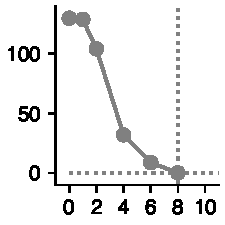
\includegraphics[width=0.98\textwidth]{figures/evaluateCrossValidationResults_Synthetic_Gardelle.py_SimulateSynthetic_Parameterized_OtherNoiseLevels_Grid_VarySize.py_180_8_2345_N10000_FOURIER_183_FOURIER_283.txt_RelativeLF.pdf}
\end{minipage}

\caption{Supplement to Figure 4: Randomly constructed models.
We simulate three models at the ground truth loss function exponent indicated.
The loss function is clearly identified by model fit, and, when fitting at this loss, prior and encoding are recovered.
See Section~\ref{sec:att-rep} for discussion of Attraction and Repulsion components.
}
\label{fig:fourier-8}
\end{figure}


